% %%%%%%%%%%%%%%%%%%%%%%%%%%%%%%%%%%%%%%%%%%%%%%%%%%%%%%%%%%%%%%%%%%%%%%%%%%%%%%%%%
The influence of the freshwater discharged to the Oslofjord by way of the many rivers surrounding it is well known. A relevant example is shown by Figure \ref{fig:salt_hele} constructed from a test run with an earlier version of the FjordOs CL model. In particular the impact on the daily mean sea surface salinity of Norway's two largest rivers, namely Glomma to the southeast and Drammenselva to the northwest, is evident. As shown it tends to create salinity fronts that in turn give rise to high lateral as well as vertical shear currents. From time to time these fronts are even strong enough to generate instabilities. To obtain a realistic, high resolution picture of the circulation in the Oslofjord it is therefore paramount to include the input from these and other smaller rivers.
%%%%%%%%%%%%%%%%%%%%%%%%%%%% Figure 13 FjordOs salinity %%%%%%%%%%%%%%%%%%%%
\begin{figure}[t]
 \begin{center}
  \begin{pspicture}(0,0)(15,12)
   \rput[b]( 7.5,0.0){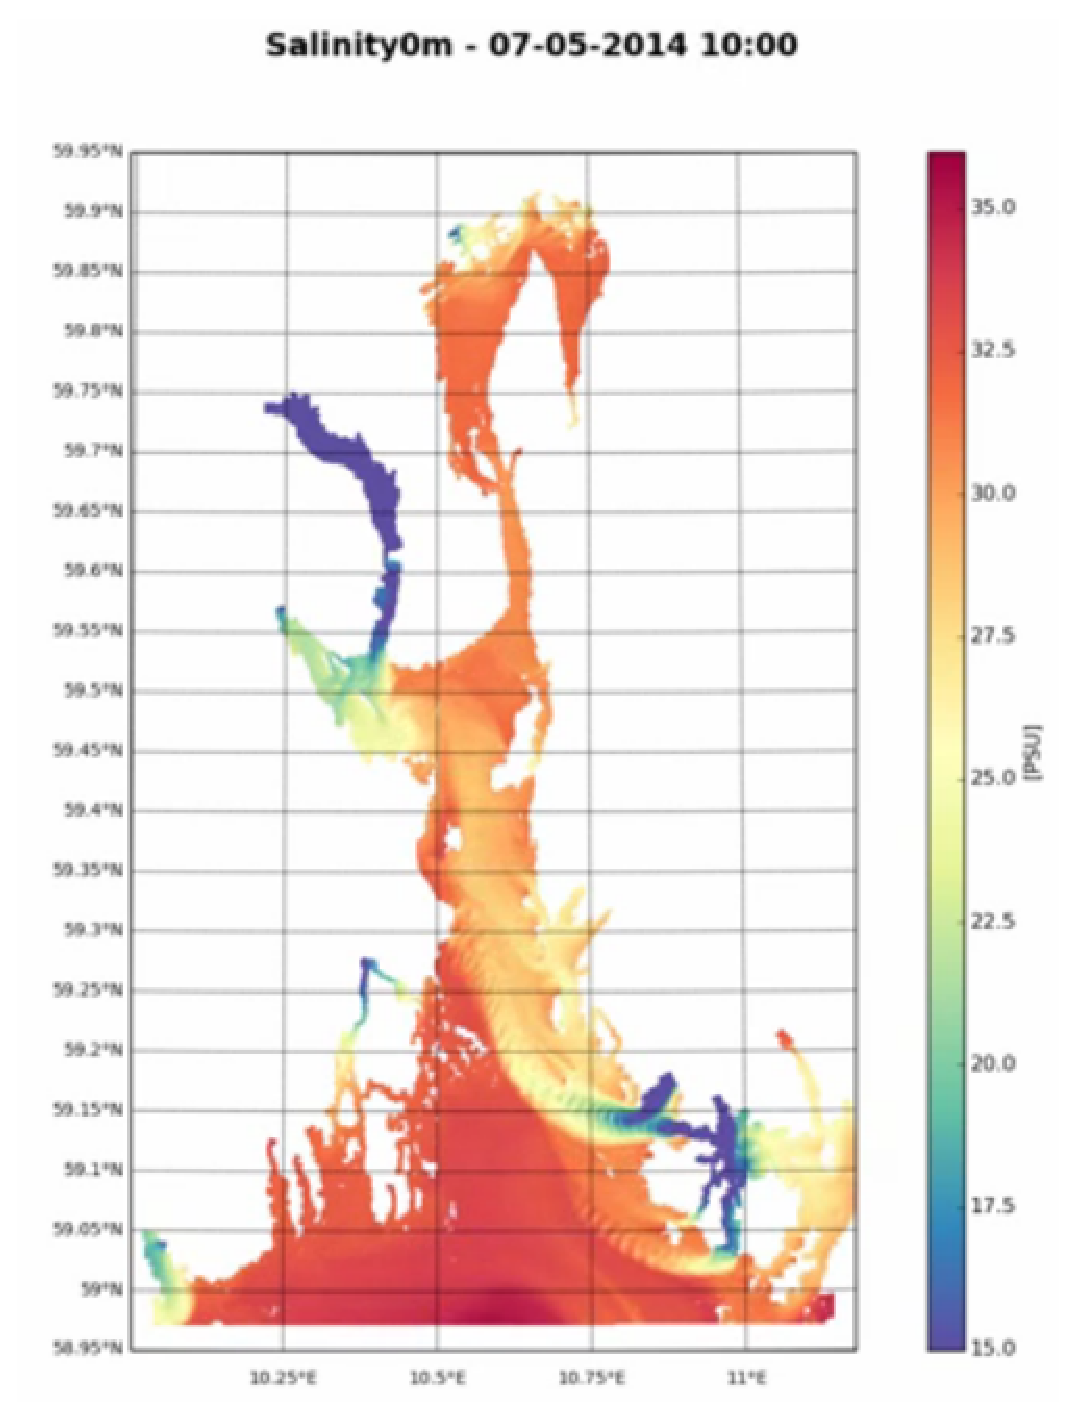
\includegraphics[height=12cm]{fjordos_salinity}}
  \end{pspicture}
  \caption{\small Daily mean sea surface salinity valid at May 7, 2014 from an earlier testrun. The color bar gives salinity in units of psu. Longitude and latitude are indicated along the axes. Note the impact of the freshwater discharged by the major rivers on the salinity, and the tendency of the Coriolis effect to turn the freshwater flux from Glomma northward.} 
  \label{fig:fjordos_salinity}
 \end{center}
\end{figure}


% %%%%%%%%%%%%%%%%%%%%%%%%%% Figure 1 Oversiktskart %%%%%%%%%%%%%%%%%%%%%%%%%%%%
\begin{figure}[t]
 \setlength{\unitlength}{1.0cm}
 \begin{center}
  \begin{pspicture}(0,0)(15,9)
% Include graphs
   \rput[bl](0,0){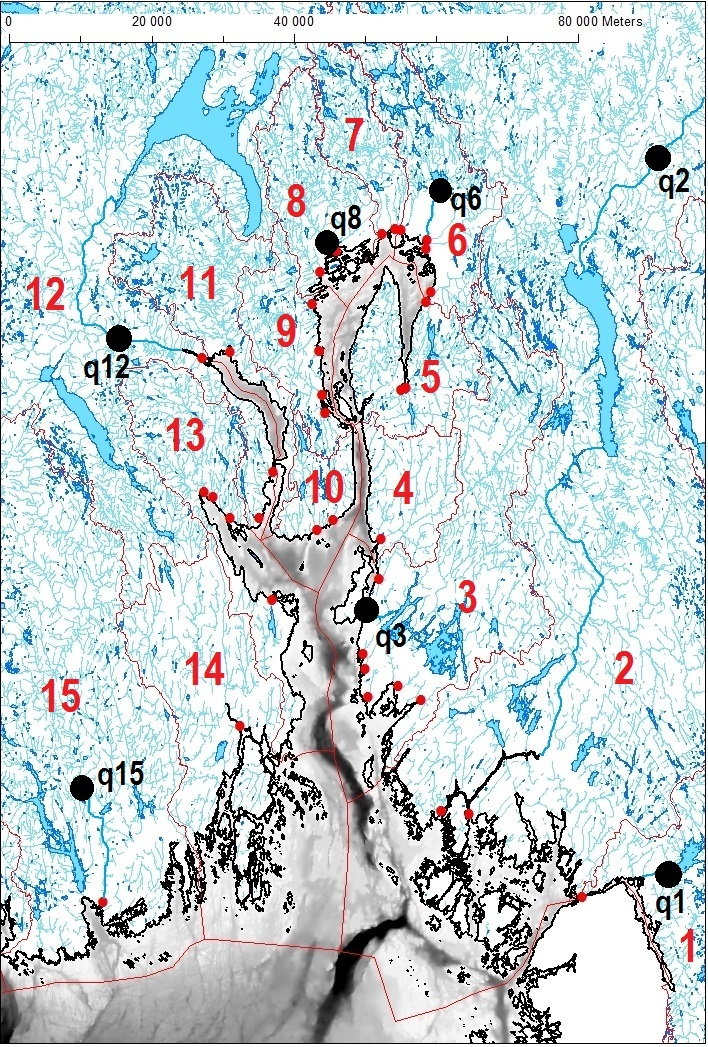
\includegraphics[height=9cm]{Elver_Oslofjorden_v4}}
   \rput[br](15,0){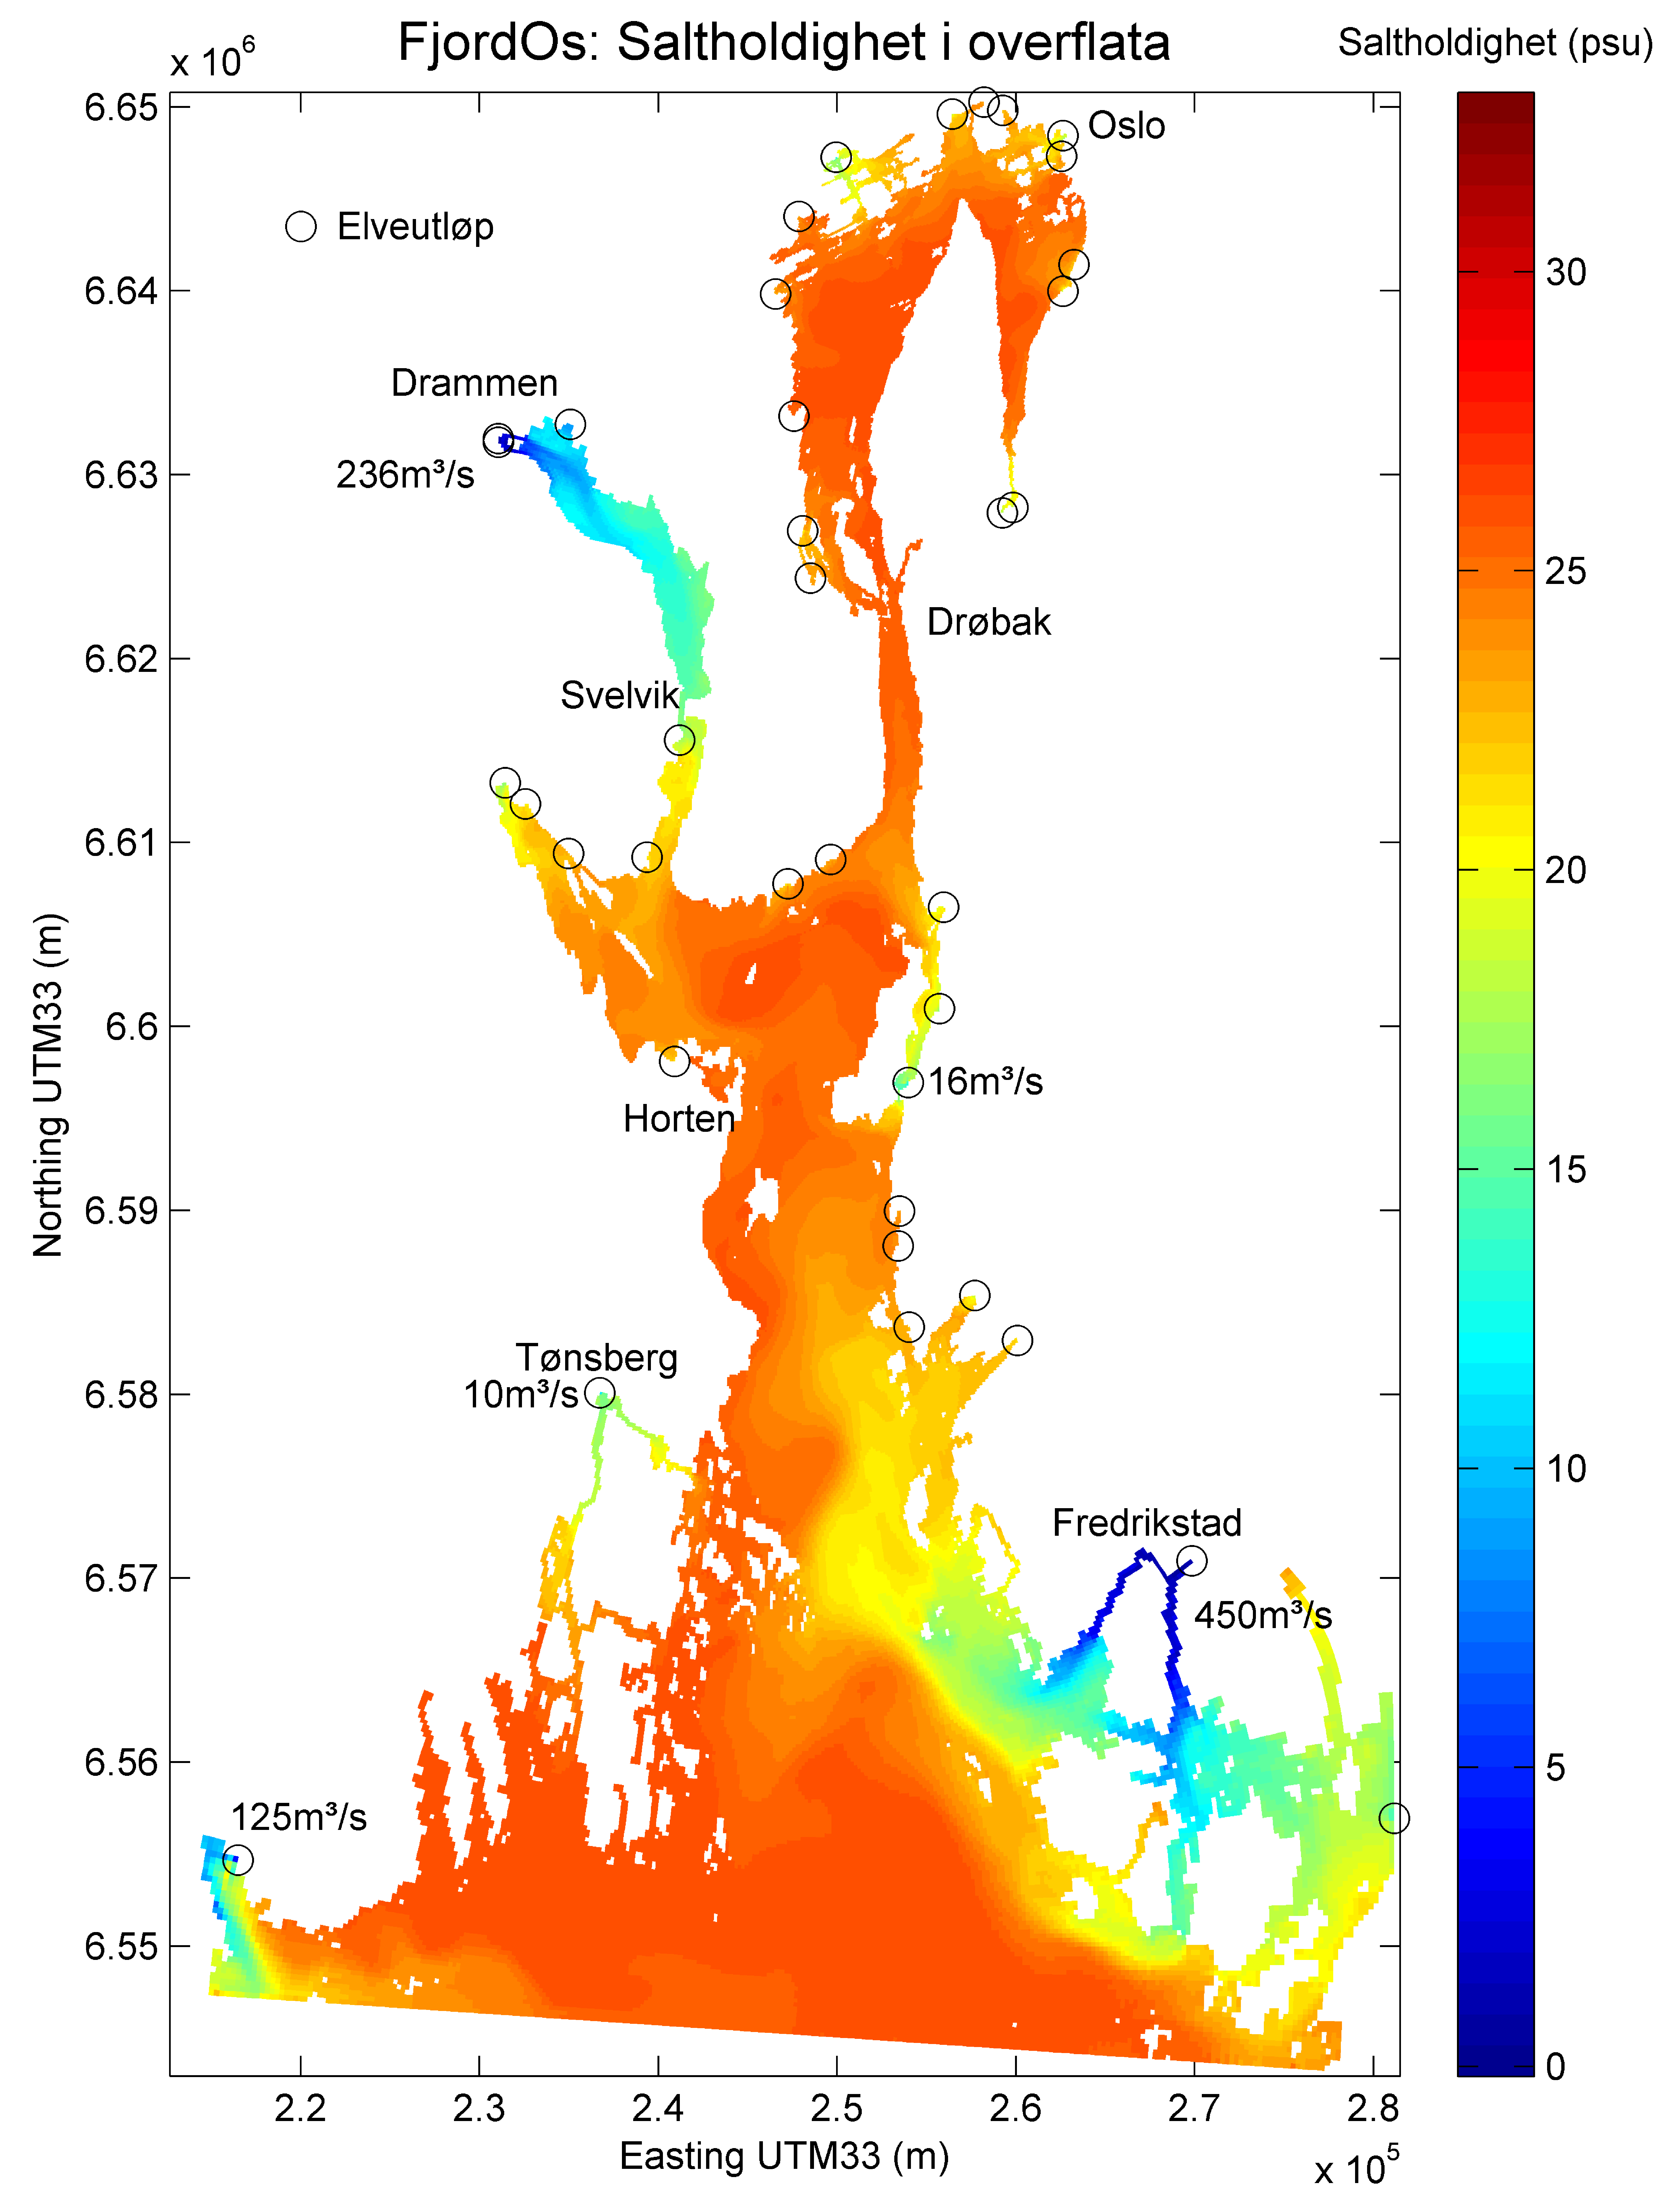
\includegraphics[height=9cm]{fjordos_rivers}}
  \end{pspicture}
% Figure caption is below the figure
  \caption{Left panel shows the many rivers (blue solid lines) emptying freshwater to the fjord (from NVE elvenett). The red numbers indicate a Main Catchment Area (MCA). The red dots indicate the location of the individual rivers discharging freshwater to Oslofjord (cf. Table \ref{tab:rivers01}). Some of the larger rivers, for instance Glomma, Drammenselva and Numedalsl{\aa}gen, are marked with a thicker blue line. Stations with water discharge measurements are shown with green dots and numbered with black numbers, e.g. q8. Right panel shows the location of the 37 rivers named in Table \ref{tab:rivers01}. }   
  \label{fig:rivers01}      
 \end{center}
\end{figure}
%

 

To obtain the necessary information on the freshwater discharges to the Oslofjord within the FjordOs CL model domain we make use of discharge data from a database constructed by use of the hydrological model HBV \citep{beldr:etal:2003}. In essence the HBV model provides an estimate of the daily mean freshwater drained into the ocean (or fjord) from a preselected set of so called Main Catchment Areas (MCAs). Each MCA has in turn at least one or more rivers with an outlet to the sea. Let $Q_i$ be the daily mean freshwater discharged from the $i$th MCA and $A_i$ its area. Furthermore, let $q_{ij}$ be the discharge from the $j$th individual river associated with the $i$th MCA. Then assuming that $q_{ij}$ is entirely determined by the ratio of its local catchment area $a_{ij}$ to the area of the MCA, that is $A_i$ we get
\be
 \label{eq:riv02}
  q_{ij} = \frac{a_{ij}}{A_i} Q_i.
\ee

A total of 15 of Norway's MCAs drains into the Oslofjord within the FjordOs model domain (Figure \ref{fig:rivers01}). These MCAs in turn contain a total of 46 river outlets as listed by Table \ref{tab:rivers01}. Six of these belongs to Glomma and five to Drammenselva. Hence there are 37 named rivers. Their locations are shown by Figure \ref{fig:rivers01}. By use of (\ref{eq:riv02}) and Table \ref{tab:rivers01} we may find the discharge emitted from each of them provided $Q_i$ is known. The HBV database contains information on $Q_i$ from 1962 up to and including the previous year with a lag of about six months. Thus $Q_i$ is not available for 2015 yet. Our hindcast period is from April 1, 2014 up to and including December 2015. We must therefore obtain information on $Q_i$ for 2015 from another source. To this end we make use of observations from the NVE website\footnote{\texttt{http://www2.nve.no/h/hd/plotreal/Q/index.html}} available in near real time. If we for instance consider the observed discharge from river $n$ within the $i$th MCA, we find $Q_i$ by rearranging (\ref{eq:riv02}), that is,
\be
 \label{eq:riv03}
  Q_i = A_i\frac{q_{in}}{a_{in}}.
\ee
where $q_{in}$ is the known discharge of the $n$'th river and $a_{in}$ is the size of its local catchment area. Having thus found $Q_i$ we find the discharges from the remaining rivers of that MCA by use of (\ref{eq:riv02}) and the $a_{ij}$'s listed in Table \ref{tab:rivers01}.

Using this method we first calculated the daily mean discharge for MCA numbers $i=1, 2, 3, 6, 8, 12$, and $15$ using the NVE station data for rivers nos. 1 (Iddefjorden/Haldenv.), 2-7 (Glomma), 13 (Mosseelva), 21 (Akerselva), no. 25 (Sandvikselva), 34-38 (Drammenselva) and 46 (Numedalsl{\aa}gen). The NVE station for MCA no. 2 is located far upriver (Figure \ref{fig:rivers01}), so a correction factor is estimated based on a least square fit between the NVE observations at R{\aa}n{\aa}sfoss and the Glommens og Laagens Brukseierforening (glb.no) observations at Sarpfoss for the period up to and including October 28, 2015. The result is
\be
 \label{eq:riv04}
 Q_2 = 1.123 \cdot Q_{\text{R{\aa}n{\aa}sfoss}}.
\ee
This yields an estimate of the river discharge in Glomma with an RMS error of about 100 m$^3$/s. The corresponding discharges, that is, $q_{2j}$ for $j=2,3,\ldots,7$, are found by use of (\ref{eq:riv02}) and the size of the corresponding local catchment areas $a_{2j}$ listed in Table \ref{tab:rivers01}.
%%%%%%%%%%%%%%%%%%%%%%%%%%% Location of rivers %%%%%%%%%%%%%%%%%%%%%%%%%%%%%%%%%%%%%%
\clearpage
\vspace{5mm}
\tablecaption{Rivers in the FjordOs CL model. The outlet positions follow the index convention in ROMS. The position is at a $u$-point if the direction is along the $x$-axis, and at a $v$-point if the direction is along the $y$-axis. The index counting in ROMS starts at 0, except for the $u$-points and $v$-points, where the count starts at 1. MCA: Main Catchment Area.}
\tablefirsthead{\hline 
  River	& MCA	& \mc{1}{c}{Area}	& Outlet	& Outlet	& Direction	& Sign	& Name			\\ 
  No.	& no.   & \mc{1}{c}{$a_{ij}$}	& $x$-pos.	& $y$-pos.	& 0=along $x$	&	&			\\
	&       &			&       	&       	& 1=along $y$	&	&			\\
		\hline }
\tablehead{\hline \mc{8}{l}{\small\slshape continued from previous page}  \\ \hline
  River	& MCA	& \mc{1}{c}{Area}	& Outlet	& Outlet	& Direction	& Sign	& Name			\\ 
  No.	& no.   & \mc{1}{c}{$a_{ij}$}	& $x$-pos.	& $y$-pos.	& 0=along $x$	&	&			\\
	&       &			&       	&       	& 1=along $y$	&	&			\\
		\hline}
\tabletail{\hline \mc{8}{r}{\small\slshape continued on next page}  \\ \hline}
\tablelasttail{\hline}
\begin{center}
% \newcolumntype{d}{D{.}{.}{2}}
 \begin{supertabular}{ccrccccl}
  1	& 1	& 2512.00	& 297		& 44		& 0		& -1	& Iddefjorden/Haldenv.		\\
  2	& 2	& 7222.43	& 261		& 77		& 1		& -1	& Glomma ({\O}sterelva)		\\
  3	& 2	& 7222.43	& 260		& 77		& 1		& -1	& Glomma ({\O}sterelva)		\\
  4	& 2	& 7222.43	& 259		& 77		& 1		& -1	& Glomma ({\O}sterelva)		\\
  5	& 2	& 7222.43	& 258		& 70		& 1		& -1	& Glomma ({\O}sterelva)		\\
  6	& 2	& 7114.64	& 248		& 91		& 0		& -1	& Glomma (Vesterelva)		\\
  7	& 2	& 7114.64	& 248		& 92		& 0		& -1	& Glomma (Vesterelva)		\\
  8	& 3	& 13.90		& 273		& 202		& 0		& -1	& Krokstadbekken		\\
  9	& 3	& 25.90		& 251		& 230		& 1		& -1	& Heiabekken+Kure{\aa}a		\\
  10	& 3	& 7.57		& 213		& 219		& 1		& -1	& St{\o}tvikbekken		\\
  11	& 3	& 3.83		& 211		& 258		& 1		& +1	& Evje{\aa}a			\\
  12	& 3	& 5.55		& 213		& 275		& 1		& -1	& Gunnarbybekken		\\
  13	& 3	& 688.34	& 221		& 337		& 0		& -1	& Mossevassdraget		\\
  14	& 3	& 19.33		& 239		& 373		& 0		& -1	& Kambobekken			\\
  15	& 4	& 138.49	& 242		& 423		& 0		& -1	& H{\ae}lenelva			\\
  16	& 5	& 6.94		& 273		& 634		& 1		& +1	& Gloslibekken			\\
  17	& 5	& 51.72		& 280		& 638		& 1		& +1	& {\AA}rungelva			\\
  18	& 5	& 85.97		& 286		& 784		& 0		& -1	& Gjersj{\o}elva		\\
  19	& 6	& 39.10		& 289		& 802		& 0		& -1	& Ljanselva			\\
  20	& 6	& 69.26		& 267		& 864		& 0		& -1	& Alna				\\
  21	& 6	& 237.81	& 266		& 876		& 1		& -1	& Akerselva                	\\
  22	& 6	& 23.24		& 226		& 890		& 1		& -1	& Frognerbekken            	\\
  23	& 7	& 14.46		& 213		& 895		& 0		& -1	& Hoffelva               	\\
  24	& 7	& 176.30	& 188		& 888		& 1		& -1	& Lysakerelva                	\\
  25	& 8	& 227.72	& 83		& 843		& 1		& -1	& Sandvikselva                 	\\
  26	& 8	& 21.74		& 72		& 782		& 1		& -1	& Neselva			\\
  27	& 9	& 37.63		& 84		& 726		& 1		& +1	& Askerelva                   	\\
  28	& 9	& 2.82		& 126		& 665		& 1		& +1	& N{\ae}rsneselva		\\
  29	& 9	& 112.95	& 149		& 607		& 0		& +1	& {\AA}rosvassdraget		\\
  30	& 9	& 19.05		& 158		& 584		& 0		& +1	& S{\ae}treelva               	\\
  31	& 10	& 18.01		& 179		& 447		& 1		& -1	& Tofteelva			\\
  32	& 10	& 35.47		& 156		& 435		& 1		& -1	& Sageneelva			\\
  33	& 11	& 309.38	& 22		& 621		& 1		& -1	& Lierelva			\\
  34	& 12	& 2139.31	& 1		& 611		& 0		& +1	& Drammeneslva 1		\\
  35	& 12	& 4278.61	& 1		& 610		& 0		& +1	& Drammenselva 2		\\
  36	& 12	& 4278.61	& 1		& 609		& 0		& +1	& Drammenselva 3		\\
  37	& 12	& 4278.61	& 1		& 608		& 0		& +1	& Drammenselva 4		\\
  38	& 12	& 2139.31	& 1		& 607		& 0		& +1	& Drammeneslva 5		\\
  39	& 12	& 8.11		& 97		& 501		& 1		& -1	& Ebbestadelva   		\\
  40	& 12	& 14.54		& 82		& 447		& 0		& +1	& Bergerelva    		\\
  41	& 13	& 6.59		& 42		& 450		& 1		& -1	& Sandobekken    		\\
  42	& 13	& 29.84		& 22		& 472		& 1		& -1	& Selvikelva  			\\
  43	& 13	& 193.23	& 13		& 481		& 1		& -1	& Sandevassdraget   		\\
  44	& 13	& 33.66		& 93		& 351		& 1		& +1	& Borreelva       		\\
  45	& 14	& 1115.00	& 61		& 186		& 0		& +1	& Aulivassdraget      		\\
  46	& 15	& 6514.00	& 9		& 23		& 0		& -1	& Numedalsl{\aa}gen  		\\
 \end{supertabular}
\label{tab:rivers01}
\end{center}
\vspace{5mm}



For some of the 15 MCAs in the model domain, no observations are available ($i=$ 4, 5, 7, 9, 10, 11, 13, 14). We have estimated $Q_i$ for these rivers using the $Q_i$'s from MCA nos. 2 (Glomma), 3 (Mosseelva), 8 (Sandvikselva) and 15 (Nummedalsl{\aa}en). An auxiliary parameter was calculated that was the sum of the river discharges of all combinations of the four rivers. A least mean square fit was performed between this new parameter and the discharge for the MCA in question, namely 
\be
 \label{eq:riv05}
 Q_i = \alpha_i \left(f_{i2} Q_2 + f_{i3} Q_3 + f_{i8} Q_8 +f_{i15} Q_{15}\right) + \beta_i .
\ee
The result of this analysis is shown in Table \ref{tab:rivers04}. It is somewhat surprising that the discharge from MCA nos. 2 and 15 did not influence the estimate of the discharge from the other MCAs.   
%%%%%%%%%%%%%%%%%%%%%%%%%%% Summary of experiments %%%%%%%%%%%%%%%%%%%%%%%%%%%%%%%%%%%%%%
%\clearpage
\begin{table}[t]
 \caption{Estimating discharges in unobserved MCAs based on observations
 at four MCAs with observations using the least mean square fit (\ref{eq:riv05}).}
 \label{tab:rivers04}       % Give a unique label
% For LaTeX tables use
 \centering
% \begin{center}
   \begin{tabular}{ccccccc}
   \hline
   MCA & $f_{i2}$ & $f_{i3}$ & $f_{i8}$ & $f_{i15}$ & $\alpha_i$ & $\beta_i$  \\
   no. &          &          &          &           &            &            \\ 
   \hline
   4   & 0        &  1       &  0       &  0        & 0.201      &  0.120     \\
   5   & 0        &  1       &  0       &  0        & 0.265      &  0.274     \\
   7   & 0        &  0       &  1       &  0        & 0.625      &  0.531     \\
   9   & 0        &  0       &  1       &  0        & 0.750      &  0.209     \\
   10  & 0        &  0.5     &  0.5     &  0        & 0.264      & -0.276     \\
   11  & 0        &  0       &  1       &  0        & 1.317      &  0.417     \\
   13  & 0        &  0       &  1       &  0        & 1.081      &  0.998     \\
   14  & 0        &  0.5     &  0.5     &  0        & 1.000      &  1.087     \\
   \hline
   \end{tabular}
% \end{center}
\end{table}



Finally we emphasize that the rivers, in addition to providing freshwater to the fjord, are sources of nutrients, organic matter, bacteria, particles and contaminants. Several of these parameters are monitored in the national monitoring program \citep[Riverine Inputs and direct Discharges - RID,][]{skarb:etal:2011}. It is therefore possible to include information from the RID program in the river forcing, and hence the FjordOs CL model may be used in the future to model dispersion of any of the RID parameters.





